\documentclass[
		11pt,
		a4paper,
		toc=listof, %% Abbildungs-, Tabellenverzeichnis mit ins Inhaltsverzeichni
		bibliography=totoc %% Quellenverzeichnis mit ins Inhaltsverzeichnis
		]{scrreprt}	 %% KOMA Script

% HTWG
\usepackage{graphicx}
\usepackage{a4}
\usepackage{german}

% Eigene
\usepackage[utf8]{inputenc} %% Umlaute
\usepackage[printonlyused]{acronym} %% Abkuerzungsverzeichnis (nur verwendete)
\usepackage{todonotes} %% TODOs moeglich mit \todo{}
\usepackage{booktabs} %% Tabellen
\usepackage{amsmath} %% Formeln
\usepackage{listings} %% Codebeispiele
\usepackage{subfigure} %% Mehrere Bilder nebeneinander
\usepackage{hyperref} %% referenzen innerhalb und außerhalb des Dokumentes

% Eigenes Design
%TODO loeschen wenn default HTWG Design (was es nicht wirklich gibt) gewuuenscht ist
\usepackage[bottom=3cm]{geometry}
\usepackage{setspace}
\onehalfspacing


% KOMA script anpassungen
%TODO entfernen wenn kein KOMA Script gewuenscht
\usepackage{scrhack}

%%%%%%%% Codebeispiele
\usepackage{color}
\usepackage{xcolor}
\usepackage{listings}
\usepackage{caption}

\setcounter{tocdepth}{2}  %% Uebreschriften bis subsectionw ins Inhaltsverzeichnis
\setcounter{secnumdepth}{2}  %% Nummerierung bis subsection


%%% Codebeispiele - Style
\lstdefinestyle{mystyle}{
    basicstyle=\footnotesize,
    aboveskip=10pt,
    breakatwhitespace=false,
    breaklines=true,
    captionpos=b,
    belowcaptionskip=5pt,
    keepspaces=true,
    numbers=left,
    numbersep=15pt,
    showspaces=false,
    showstringspaces=false,
    showtabs=false,
    tabsize=2,
    frame=single,
    lineskip=-0.4pt,
    framexleftmargin=0.5em,
    xleftmargin=2.5em
}
\lstset{style=mystyle}


% Entfernt Kapitel Ueberschrift
% Bsp.
% 	ALT:
%       Kapitel 1
%       Einführung
%
% 	NEU:
% 		1 Einführung
%
\renewcommand*\chapterheadstartvskip{\vspace{-\topskip}}


% Hurenkind und Schusterjunge vermeiden
\clubpenalty = 10000 % schliesst Schusterjungen aus
\widowpenalty = 10000 \displaywidowpenalty = 10000% schliesst Hurenkinder aus


% Alle Listen mit einem "-" statt einem Punkt
\def\labelitemi{--}


\newcommand{\thema}{$[$Thema der Bachelorarbeit$]$}
\newcommand{\schlagworte}{$[$Platz, f\"ur, spezifische, Schlagworte, zur, Ausarbeitung $]$}
\newcommand{\zusammenfassung}{$[$Text der Zusammenfassung etwa 150 Worte. Es soll der
	L"osungsweg beschrieben sein.$]$}
\newcommand{\ausgabedatum}{$[$Datum$]$}
\newcommand{\abgabedatum}{15.02.2016}
\newcommand{\autor}{Sandro Tonon}
\newcommand{\autorStrasse}{Allemannenstra"se 10}
\newcommand{\autorPLZ}{78467}
\newcommand{\autorOrt}{Konstanz}
\newcommand{\autorGeburtsort}{Waldshut-Tiengen}
\newcommand{\autorGeburtsdatum}{02.07.1990}
\newcommand{\prueferA}{Prof. Dr. Marko Boger}
\newcommand{\prueferB}{Dipl. Ing. Andreas Maurer}
\newcommand{\firma}{Seitenbau GmbH}
\newcommand{\studiengang}{Angewandte Informatik}



\begin{document}
%% Nummerierung aus
\pagenumbering{gobble}

% HTWG Tempaltes fuer Titelseite etc.

\begin{titlepage}

\vspace*{-3.5cm}

\begin{flushleft}
\hspace*{-1cm} 
\includegraphics[width=15.7cm]{htwg-logo}
\end{flushleft}

\vspace{2.5cm}

\begin{center}
	\huge{
		\textbf{\thema} \\[5cm]
	}
	\Large{
		\textbf{\autor}} \\[6.5cm]
	\large{
		\textbf{Konstanz, \abgabedatum} \\[2.3cm]
	}
	
	\Huge{
		\textbf{{\sf BACHELORARBEIT}}
	}
\end{center}

\end{titlepage}

\thispagestyle{empty}
{
\setlength{\parskip}{0.5cm}
        \begin{center}
        \textbf{\huge BACHELORARBEIT}

        \textbf{zur Erlangung des akademischen Grades}

        \textbf{\Large Bachelor of Science (B. Sc.)}

        \textbf{an der}

        \textsf{\huge Hochschule Konstanz}\\
        {\small Technik, Wirtschaft und Gestaltung}

        \textsf{\Large Fakult"at Informatik} \\
        Studiengang \studiengang
        \end{center}
}
\begin{center}

\vspace*{2cm}

\begin{tabular}{p{3cm}p{10cm}}
Thema: & \multicolumn{1}{l}{\textbf{\large \thema}} \\[15ex]
Bachelorkandidat: & \autor, \autorStrasse, \autorPLZ{}  \autorOrt{} \\[15ex]
1. Pr"ufer: & \prueferA \\
2. Pr"ufer: & \prueferB \\[25ex]
Ausgabedatum: & \ausgabedatum \\
Abgabedatum: & \abgabedatum \\
\end{tabular}
\end{center}

\begin{center}
{\Large \textbf{Zusammenfassung (Abstract)}}
\end{center}

\bigskip

\begin{center}
	\begin{tabular}{p{2.8cm}p{10cm}}
		Thema: & \thema \\
		 & \\
		Bachelorkandidat: & \autor \\
		 & \\
		Firma: & \firma \\
		 & \\
		Betreuer: & \prueferA  \\[.5ex]
		 &  \prueferB \\
		 & \\
		Abgabedatum: & \abgabedatum \\
		 & \\
		Schlagworte: & \schlagworte \\
		 & \\
	\end{tabular}
\end{center}

\bigskip

\noindent
\zusammenfassung

\pagenumbering{Roman}
\chapter*{Ehrenw"ortliche Erkl"arung}
\addcontentsline{toc}{chapter}{Ehrenw"ortliche Erkl"arung}

Hiermit erkl"are ich
\textit{\autor, geboren am \autorGeburtsdatum{} in \autorGeburtsort{}}, dass ich\\

\begin{tabular}{lp{12cm}}
(1) & meine Bachelorarbeit mit dem Titel \\[1em]
& \textbf{\thema} \\[1em]
& selbstst"andig und ohne fremde Hilfe angefertigt und keine anderen als die angef"uhrten Hilfen benutzt habe;\\[1em]
(2) & die "Ubernahme w"ortlicher Zitate, von Tabellen, Zeichnungen, Bildern und
Programmen aus der Literatur oder anderen Quellen (Internet) sowie die Verwendung
der Gedanken anderer Autoren an den entsprechenden Stellen innerhalb der Arbeit
gekennzeichnet habe.\\
\end{tabular}

\vspace*{1cm}

\noindent
Ich bin mir bewusst, dass eine falsche Erkl"arung rechtliche Folgen haben wird.\\

\vspace*{3cm}

\noindent
Konstanz, \abgabedatum \hfill \begin{tabular}{c} \\ \\ \rule{5cm}{1pt} \\ (Unterschrift)\end{tabular}


\tableofcontents

% Literaturverzeichnis
\section{Abkürzungsverzeichnis}
\begin{acronym}

 \acro{bzw.}{beziehungsweise}
 \acro{HTML}{Hypertext Markup Language}
 \acro{W3C}{World Wide Web Consortium}
 \acro{DOM}{Document Object Model}
 \acro{CSS}{Cascading Style Sheets}
 \acro{API}{Application Programming Interface}
 \acro{FOUC}{Flash Of Unstyled Content}
 \acro{LIFO}{Last In First Out}

\end{acronym}
\end{document}


%% Starte Paginierung
\cleardoublepage
\pagenumbering{arabic}


%!TEX root = ../thesis.tex

\chapter{Grundlagen}

\ac{LOL} Lorem ipsum dolor sit amet, consetetur sadipscing elitr, sed diam nonumy eirmod tempor invidunt ut labore et dolore magna aliquyam erat, sed diam voluptua. At vero eos et accusam et justo duo dolores et ea rebum. Stet clita kasd gubergren, no sea takimata sanctus est Lorem \ac{HTTP} ipsum dolor sit amet. Lorem ipsum dolor sit amet, consetetur sadipscing elitr, sed diam nonumy eirmod tempor invidunt ut labore et dolore magna aliquyam erat, sed diam voluptua. At vero eos et accusam et justo duo dolores et ea rebum. Stet clita kasd gubergren, no sea takimata sanctus est Lorem ipsum dolor sit amet.

\section{tbd} 

Lorem ipsum dolor sit amet, consetetur sadipscing elitr, sed diam nonumy eirmod tempor invidunt ut labore et dolore magna aliquyam erat, sed diam voluptua. At vero eos et accusam et justo duo dolores et ea rebum. Stet clita kasd gubergren, no sea takimata sanctus est Lorem ipsum dolor sit amet. Lorem ipsum dolor sit amet, consetetur sadipscing elitr, sed diam nonumy eirmod tempor invidunt ut labore et dolore magna aliquyam erat, sed diam voluptua. At vero eos et accusam et justo duo dolores et ea rebum. Stet clita kasd gubergren, no sea takimata sanctus est Lorem ipsum dolor sit amet.

\subsection{tbd} 
Lorem ipsum dolor sit amet, consetetur sadipscing elitr, sed diam nonumy eirmod tempor invidunt ut labore et dolore magna aliquyam erat, sed diam voluptua. At vero eos et accusam et justo duo dolores et ea rebum. Stet clita kasd gubergren, no sea takimata sanctus est Lorem ipsum dolor sit amet. Lorem ipsum dolor sit amet, consetetur sadipscing elitr, sed diam nonumy eirmod tempor invidunt ut labore et dolore magna aliquyam erat, sed diam voluptua. At vero eos et accusam et justo duo dolores et ea rebum. Stet clita kasd gubergren, no sea takimata sanctus est Lorem ipsum dolor sit amet.

\subsubsection{tbd} 
Lorem ipsum dolor sit amet, consetetur sadipscing elitr, sed diam nonumy eirmod tempor invidunt ut labore et dolore magna aliquyam erat, sed diam voluptua. At vero eos et accusam et justo duo dolores et ea rebum. Stet clita kasd gubergren, no sea takimata sanctus est Lorem ipsum dolor sit amet. Lorem ipsum dolor sit amet, consetetur sadipscing elitr, sed diam nonumy eirmod tempor invidunt ut labore et dolore magna aliquyam erat, sed diam voluptua. At vero eos et accusam et justo duo dolores et ea rebum. Stet clita kasd gubergren, no sea takimata sanctus est Lorem ipsum dolor sit amet.


%!TEX root = ../thesis.tex

\chapter{Codebeispiel}

Lorem ipsum dolor sit amet, consetetur sadipscing elitr, sed diam nonumy eirmod tempor invidunt ut labore et dolore magna aliquyam erat, sed diam voluptua. At vero eos et accusam et justo duo dolores et ea rebum. Stet clita kasd gubergren, no sea takimata sanctus est Lorem ipsum dolor sit amet. Lorem ipsum dolor sit amet, consetetur sadipscing elitr, sed diam nonumy eirmod tempor invidunt ut labore et dolore magna aliquyam erat, sed diam voluptua. At vero eos et accusam et justo duo dolores et ea rebum. Stet clita kasd gubergren, no sea takimata sanctus est Lorem ipsum dolor sit amet.

\section{tbd} 


Referenz aufs Codebeispiel \ref{code}.

\lstinputlisting[language=Java,label=code,caption=Codebeispiel Java]{kapitel3/minimalSpringBoot.java}

%!TEX root = ../thesis.tex

\chapter{Bilder}

Lorem ipsum dolor sit amet, consetetur sadipscing elitr, sed diam nonumy eirmod tempor invidunt 
\section{Ein Bild ganz breit} 
Verweis auf das Beispielbild \ref{fig:zuul}

\begin{figure}[htbp]
 \centering
 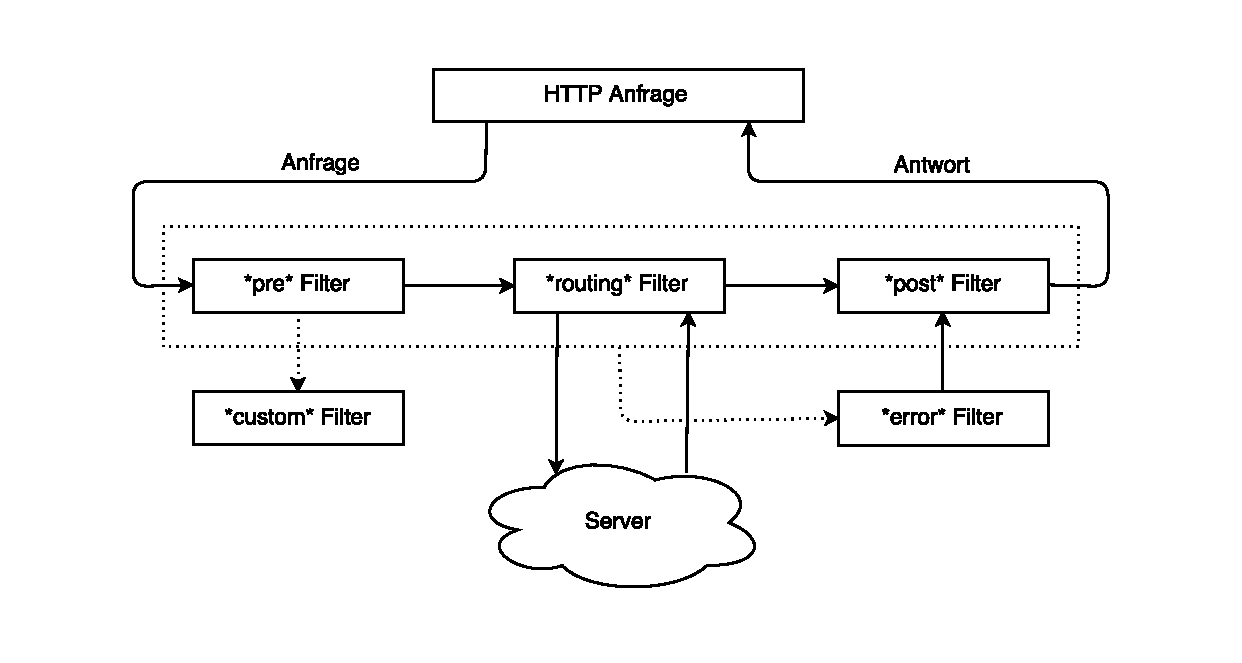
\includegraphics[width=\linewidth]{kapitel3/bilder/beispielbild}
 \caption{Beispielbild}
 \label{fig:zuul}
\end{figure}


\section{Zwei Bilder nebeneinander} 


\begin{figure}
\subfigure[Antwortzeiten]{\label{fig:antwortzeit}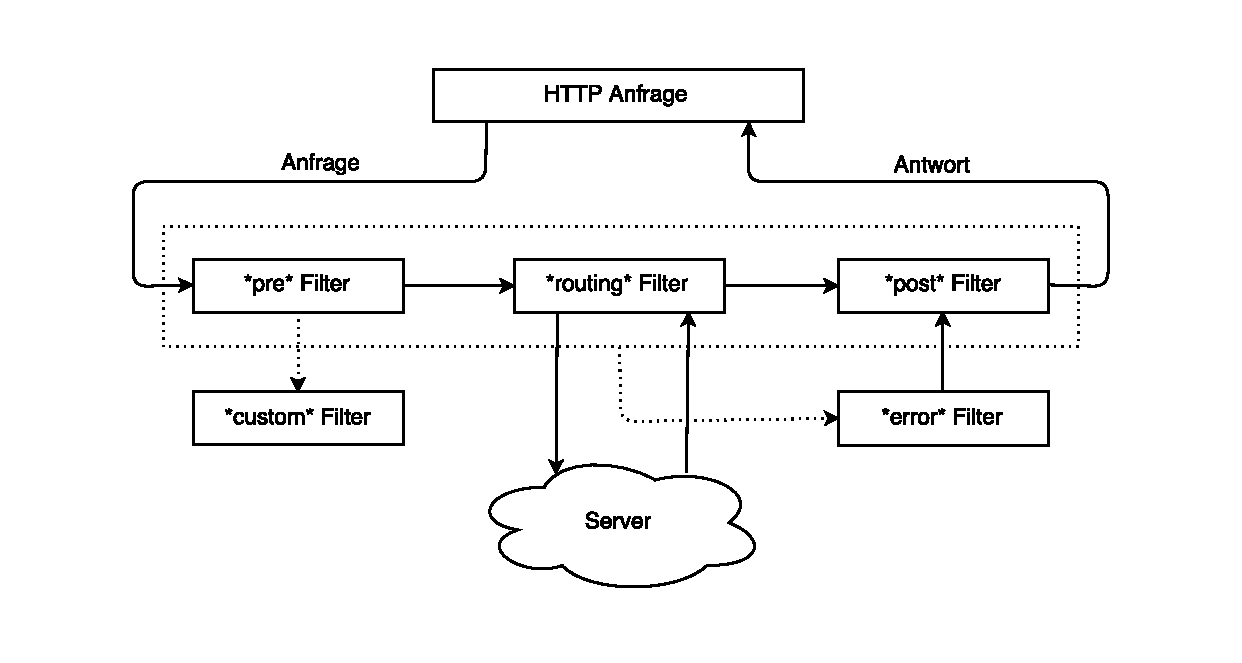
\includegraphics[width=0.50\textwidth]{kapitel3/bilder/beispielbild}}\hfill
\subfigure[prozentualer Anteil an fehlerhaften Anfragen]{\label{fig:fehler}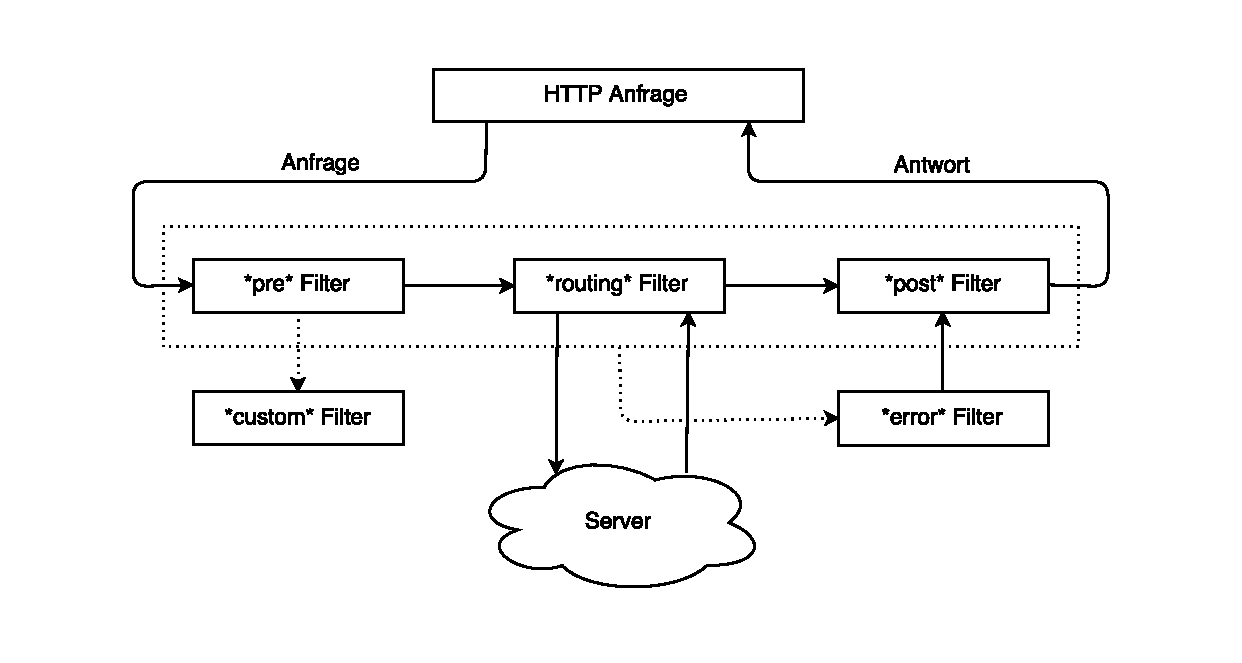
\includegraphics[width=0.50\textwidth]{kapitel3/bilder/beispielbild}}
\caption{Lasttest Szenarien}
\end{figure}

%!TEX root = ../thesis.tex

\chapter{Tabelle}

Generierbar mit \url{http://www.tablesgenerator.com/}

\section{tbd} 

\begin{table}[h]
\centering
\caption{Ergebnisse des Integartionstests in Sekunden}
\label{tab:integration}
\begin{tabular}{@{}ccccc@{}}
\toprule
Testszenario    & Start  & Registrierung & 1. Nachricht & \textbf{Gesamt} \\ \midrule
Integration\_01 & 14,598 & 10,079        & 45,449       & 70,026        \\
Integration\_02 & 14,485 & 10,108        & 54,382       & 79,088        \\
Integration\_03 & 14,498 & 10,055        & 55,125       & 79,678        \\
Integration\_04 & 14.598 & 5,361         & 36,655       & 56,614          \\ \bottomrule
\end{tabular}
\end{table}
%!TEX root = ../thesis.tex

\chapter{Quellen verwenden / verwalten}

Am besten http://www.citeulike.org/ verwenden und Expotieren als bibtex Datei.


\section{Verwenden}

Beispiel - Typ: apalike


Ergebnis: \cite{haase}


\listoffigures
\lstlistoflistings
\listoftables

% REMOVE THIS!
\listoftodos[TODOs]
% REMOVE THIS!

\bibliographystyle{apalike}
\bibliography{library}
\end{document}

